\documentclass[11pt]{article}
\usepackage{graphicx}
\usepackage{lipsum}
\usepackage{authblk}
\usepackage{titlesec}
\usepackage{multicol}
\usepackage{float}
\usepackage{geometry}

\setlength\columnsep{3em}
\setlength{\skip\footins}{2em}
\setlength{\footnotesep}{1.5em}
\geometry{
    a4paper,
    left=20mm,
    right=20mm
 }

\titleformat*{\section}{\normalsize\bfseries}
\titleformat*{\subsection}{\small\itshape}

\title{\vspace{-5em}\Huge Generation of a Synthetic Population and Travel Network for an Agent Based Traffic Simulation}
\author{\small Aniruddh Mishra, Art Barnes}
\affil{\textit{Institute for Computing in Research}}
\date{\vspace{-0.9em}\small August 2023}

\begin{document}

\maketitle

\hrule

\section*{Abstract}

\quad Traffic modeling requires various inputs to accurately simulate a real world scenario. Most traffic demand synthesis models are based on real world data, and do not reveal much information about the effects of specific attributes in cities on their traffic. By taking a set of configurations from a user, the proposed program stochastically produces a population as well as the network of a city. The program allows researchers to analyze the broad effects of city design on traffic flow, which will allow for city engineers to gain a broad understanding of how people will behave within the networks they create. With further modifications and enhancements, this software can also study the effects of different types of vehicles on carbon emissions. A possible wrapper stochastic approximation model could also determine better configurations of a given city design by interacting with this program.

\vspace{1em}

\raggedright\textit{Keywords: agent-based, zoning, graph, spanning-tree, demand, synthesis, multi-modal, stochastic}

\vspace{1em}

\hrule

\vspace{0.7em}

\begin{multicols}{2}
    \section{Introduction}
    \quad Although agent-based modeling has become increasingly popular in recent years, traffic simulations have existed for much longer. Previously, aggregate four-step models were the primary tool utilized. These models took general data of the flow of populations between zones and utilized predictive analysis techniques to determine traffic flows of the future. The main problem with this was that the models did not capture emergent effects of interactions between agents \cite{types-of-modeling}. Intuitively, this leads to several problems. First off, the lack of specific detail taken into account by these models results in simulations that simply predict patterns of groups of people. Multi-modal transportation is not captured very well in these cases. In addition, these models also don't work well with the variety of activities of different people in a population, thus they are limited by aggregate data as a whole. \\

    \quad Fortunately, nowadays, traffic simulation has started to move in the direction of agent based models \cite{ile-de-france}. These models function on a lower level, looking at the activities of people and their interactions \cite{agent-based-model}. However, in order to compute such specific predictions about a population, a lot of input data is required. Similar to any form of a simulation, you can't create information, just analyze it. Thus, the accuracy of the traffic demand determines the accuracy of the output. The best way to go about solving this problem is by sampling large populations down to an accurate, but still computable size. Still, very few governments openly release sufficient data about their populations for traffic modeling. One example, can be seen in France, where an open-source pipeline was created for this exact scenario of sampling \cite{ile-de-france}. The pipeline uses stochastic\footnote{Use of random probability to determine a quantity} models, such as the Monte Carlo simulation to sample an even size of the data of the France. In their case, the model results in data that is just 5\% of the size of Île-de-France's population. Having such a tool allows researchers to analyze existing traffic flows through agent based simulations, such as MATSIM\footnote{Open source framework for implementing agent based transport simulations} \cite{matsim}.\\

    \quad The pipeline above is one of many tools used to apply agent-based modeling to real-world scenarios. However, such methods do not allow for the analysis of hypothetical scenarios, such as variations in zoning policies. To do so, data must be manipulated and rely on the structure of a theoretical city. Unfortunately, such a program does not readily exist. In fact, prior to the publication of this paper, very few open source tools could even generate a city structure based on real-world data. Therefore, the program discussed here was created to solve this problem. Broadly speaking, it is simply a tool to generate transportation networks and traffic demand. More specifically, however, this program is intended to allow researchers and city engineers to get a general understanding of how zoning policies, network layouts, and infrastructure of transport affect the cost of construction and traffic produced within the network as a whole. To understand the functionality and structure of this program, a clear explanation of simple city structure philosophies and general graph theory will be analyzed in this paper. This will be followed by an analysis of the algorithm's implementation. Finally, we will conclude with the actual simulation and possible improvements to this model in the future.

    \section{Theory}
    \quad As stated previously, the generation of traffic demand depends on a couple of very crucial background topics. Zoning policies are very important, as they are the center of how many cities around the world are designed. This program allows for Euclidean zoning types with both hierarchical and flat zoning. The specifics of what these mean will be analyzed later, but in general both policies are very rigid. In fact, various papers link these types of zoning policies to urban sprawl \cite{zoning}. Though various other forms of zoning policies exist, euclidean zoning is by far the most popular and easy to implement.\\
    
    \quad Another topic that is very important to understand is graph theory. Having knowledge on basic graph theory will allow for a deeper intuition of how road networks are created. To allow for the configuration of the roads, a minimum spanning tree is used to create a base line infrastructure. On top of that, the networks contain meshed roads which are also subsets of the complete graph. More information will once again be analyzed, but this is one crucial implementation of Kruskal's algorithm\footnote{Algorithm to find the minimum spanning tree of a graph} in this paper. Another important use of graph theory on this project was its use for creating districts of cells in the zoning map. Rather than creating zones of all the same size, depth-first search allowed the program to make cells of a grid interconnected for more realistic zones. Once again, this will be further covered in the city zoning section, but it is a general overview of how the following theories will be applied.

    \subsection{Zoning} \label{zoning}
    
    \begin{figure}[H]
        \centering
        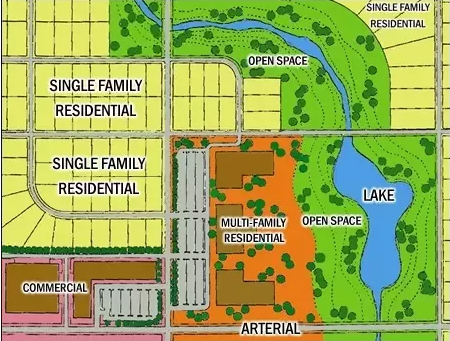
\includegraphics[width=0.4\textwidth]{images/zoning.png}
        \caption{Example zoning structure in a city \cite{zoningdiagram}}
        \label{fig:zoningdiagram}
    \end{figure}
    
    \quad When it comes to zoning, it is first crucial to understand the different types of zoning policies and their implementations in a city. First off, one of the most popular types of zoning is Euclidean zoning, which came to be known as such after its controversial use in Euclid, Ohio \cite{zoning}. This form of zoning consists of rigid divisions between types of buildings in various regions of a city. For example, residential property would be separated from commercial or industrial centers. The reasoning behind this is essentially to protect quality of living and ensure standards of health are followed. However, due to its rigid structure, the cities with heavy Euclidean zoning suffer from urban sprawl, where parts of the city continue to grow outwards. Still, within Euclidean zoning there are two variations that work differently. Hierarchical Euclidean zoning is a policy that allows for these rigid zones to be stacked upon one another. This allows for apartment complexes, for example, to exist within commercial or industrial centers. Flat zoning, on the other hand, is a standard implementation of Euclidean zoning that enforces strictly one purpose for each division of land.\\
    
    \quad The two other major forms of zoning that are newer and harder to enforce are performance based and form based zoning policies. Performance based zoning is more of a points based system that determines the criteria for a building existing within a zone as codes of compliance \cite{zoning}. These could include facilities, such as public restrooms or other standards for environmental reasons. With such a diverse and complex structure, this policy struggles to be utilized widely. Form based zoning on the other hand, is new and on the rise. This policy enforces a building's compliance through dimensions and its size \cite{zoning}. \\

    \quad Since Euclidean zoning is the most widely used and easy to regulate, our program for traffic generation is designed to study its two forms. As seen in Figure \ref{fig:zoningdiagram}, the goal of a zoning program is simply to divide up land into different shapes of various sizes. The implementation in our case went through several iterations as discussed later in section \ref{zoning-implementation}. However, the main theory that is needed to grasp the final results is based on cellular-automaton and depth first search. 

    \quad Cellular automaton was an idea thrown around to allow zoning cells to connect with one another. The pros of this idea is that it was a way to traverse the grid and set different points to a zone if not in use. As a whole, cellular automaton takes in a grid of cells and assigns values, such as on or off to these cells. Starting at a cell, the program finds its neighbors and applies a function to them to determine if their value should be changed. Now, this algorithm is actually very popular for binary systems, such as Conway's Game of Life: seen in Figure \ref{fig:cellular-automaton}. However, it tends to get very complicated very quickly when applied to a system on a higher order. Especially, a system such as configurable zoning, which does not have a finite quantity to it. If a user added more zones to the city, the program would struggle to make this functionality possible. Therefore, cellular automaton was finally determined not applicable to our zoning scenario.\\

    \begin{figure}[H]
        \centering
        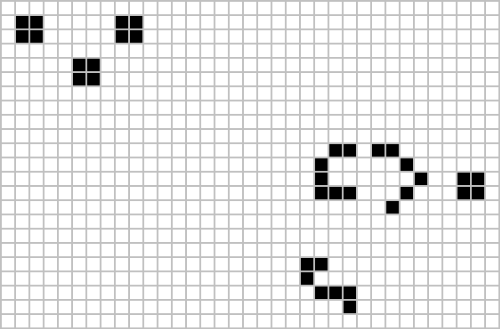
\includegraphics[width=0.4\textwidth]{images/cellularautomaton.png}
        \caption{Cellular automaton example in Conway's Game of Life \cite{cellularautomaton}}
        \label{fig:cellular-automaton}
    \end{figure}

    \quad Fortunately, the world of computer science contains various algorithms with different uses. Depth First Search\footnote{Graph theory search algorithm that is famously used in the flood fill problem} (DFS) was this magical tool for us. DFS is an algorithm in graph theory that visits starts at one node. It takes this node and randomly picks one unvisited neighbor. In our case, these nodes are cells, and the neighbors are just cells that share one edge. After picking a neighbor, the search algorithm begins again at this new cell. This cycle continues until there is a cell with no unvisited neighbors. Then, the program backtracks to the last cell with unvisited neighbors. Once the program is back at the starting cell with all other cells visited, it concludes. In our use, DFS is implented slightly differently. Rather than simply traversing our graph, we change every unvisited cell that is not already utilized by another zone to the zone that is being created. All cells that have already been assigned a zone are also considered visited neighbors. In addition, to increase randomness, this program stops after some number of iterations of not finding an unvisited cell. This means, even if the program has not concluded, if a zone is at the edge of the city, there is a chance that it won't have as many cells in it as a different district\footnote{The clump of cells in one area of a zone are called districts}. Finally, if the maximum area of a district, as defined by the configurations hsa been reached, the search terminates. Writing such an algorithm for zoning implementation may seem like a lot to do for a simple grid. However, graph theory allows programs to leverage simple mathematics to complete an otherwise daunting task, such as searching all neighboring cells.

    \begin{figure}[H]
        \centering
        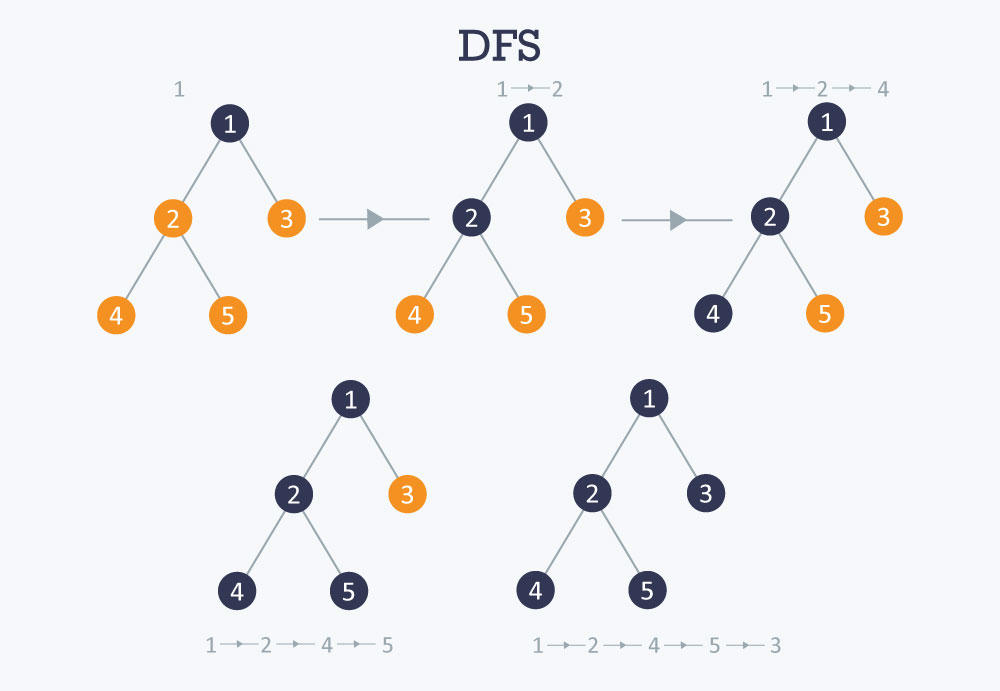
\includegraphics[width=0.45\textwidth]{images/depthfirstsearch.jpg}
        \caption{Example graph with steps of depth first search \cite{depthfirstsearch}}
        \label{fig:depth-first-search}
    \end{figure}

    \subsection{Network} \label{network}
    
    \quad Unlike zoning, making a network is actually much simpler. The two main steps comprise of creating nodes within the existing zones and making a road system that connects them together. These roads need to ensure that a person can travel from any given node to another. In our case, a node is simply a building. To determine the density of nodes in one district, several values are provided from the user's configurations. These include the average size of one building in the zone. However, this quantity is mainly used to produce the size of the zones. As far as the network goes, the generation of nodes strictly relies on the area of a building in any subzone and the area of a building in the top level zone. If no subzones are present, the types of buildings in the district will be a list of one type (the top level zone). After determining the types of buildings from the configuration file, the program randomly picks a building type and subtracts the area of it from the district's remaining area until no more buildings can be added. However, one important note is that the program also ensures that atleast one building of the top level zone's type is present. This is done by scanning neighbors, as seen in section \ref{zoning}. Once the nodes are picked out, they are converted to type Location\footnote{A class defined to make referencing node attributes easier} in the code.\\

    \quad In order to define road networks, the idea of minimum spanning trees must first be understood. Figure \ref{fig:full-graph} is an example of a graph with nodes or vertices and edges. The nodes are the points seen on the graph and the edges are the lines that link them together. There are numbers on top of each edge known as weights. In our case, higher weights represent higher distances. Figure \ref{fig:mst-graph} represents the minimum spanning tree of the former image. A spanning tree is a graph in which all nodes are connected and no cycles are formed. In particular, a minimum spanning tree is just a spanning tree with the minimum sum of weights. In our road network the baseline roads are just minimum spanning trees that connect all nodes to one another.

    \begin{figure}[H]
        \centering
        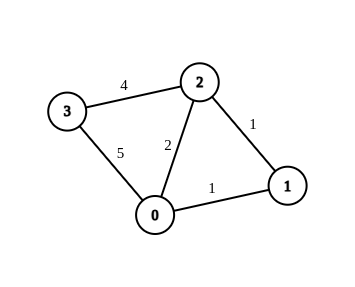
\includegraphics[width=0.45\textwidth]{images/graph.png}
        \caption{Example graph with nodes and edges \cite{graphs}}
        \label{fig:full-graph}
    \end{figure}

    \begin{figure}[H]
        \centering
        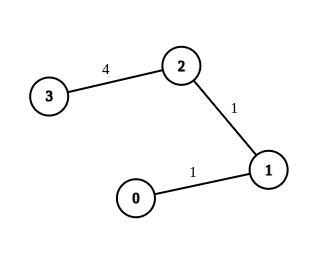
\includegraphics[width=0.4\textwidth]{images/mst.png}
        \caption{Minimum spanning tree of previous graph \cite{graphs}}
        \label{fig:mst-graph}
    \end{figure}

    \section{Implementation}

    \quad The specific implementation of these theories in our program is much simpler and easier to understand. Converting configuration data into a city structure is just a combination of the previously covered topics.
    
    \subsection{Zoning Iterations} \label{zoning-implementation}

    \begin{figure}[H]
        \centering
        \vspace{-3em}
        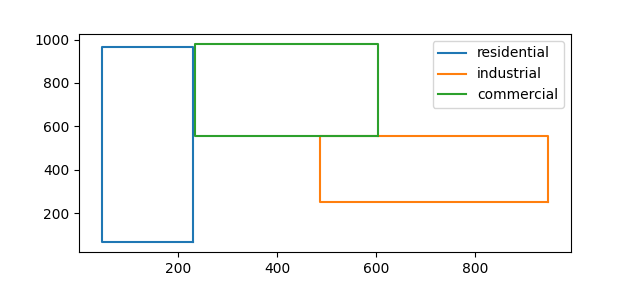
\includegraphics[width=0.45\textwidth]{images/first-zoning.png}
        \caption{First iteration of zoning}
        \label{fig:first-zoning}
    \end{figure}

    \quad Figure \ref{fig:first-zoning} illustrates the first zoning implementation of the program. This was done by taking the grid and randomly drawing a rectangle by selecting two points. These points were the top left and bottom right corners of the shape. Each rectangle was also constrained to a maximum area. This prevented the rectangle from taking over the entire plot of land. After the rectangle was created, the program selected the largest remaining plot of land. Each plot of land was defined as one edge of the existing rectangle to the end of the city. Repeating this process with the new plot of land allowed for the program to consistently draw out equal sized portions of zones. However, there were several problems with this algorithm. First off, it was overly complex. Looking for available plot of land was computer intensive and was not always guaranteed to be large enough. In addition, the rectangles did well for three zones, but quickly deteriorated after adding more. 

    \begin{figure}[H]
        \centering
        \vspace{-1em}
        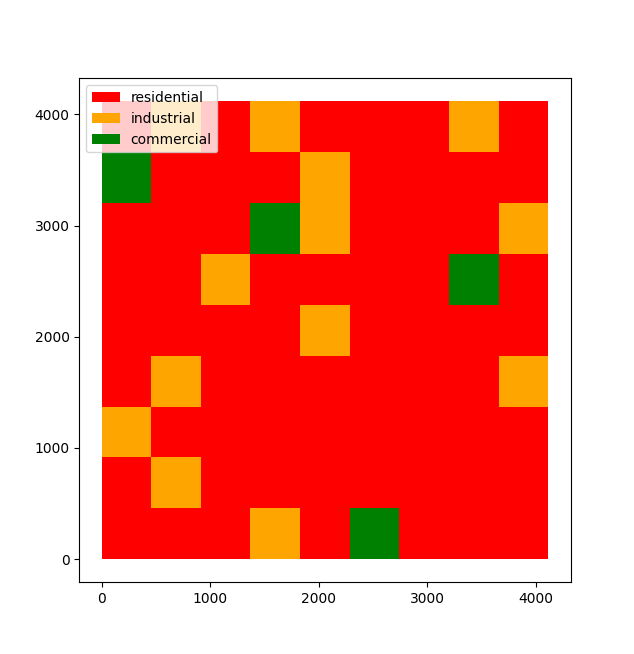
\includegraphics[width=0.45\textwidth]{images/secondzoning.png}
        \caption{Second iteration of zoning}
        \label{fig:second-zoning}
    \end{figure}

    \quad Figure \ref{fig:second-zoning} is a much better representation of zoning policies in a city. It looks a lot closer to Figure \ref{fig:zoningdiagram}. This was achieved by dividing the land into cells on a grid. The size of a cell was the minimum size of a district in a zone. One district's size was determined with the following formula: 

    \[A = B \cdot M\]

    In this formula, A represents the area of a district, B is the average size of a building in a given zone, and M is the minimum number of buildings within a district. After computing A for every zone, the algorithm picked out the minimum area of a district and set the cell length to \(\sqrt{A}\). This method worked fairly well, but still had several issues. For one, the zones were all of the same size blocks. Also, apart from the predominant zone, all the other districts were usually one block large. In most modern cities, the size of a district depends on its zone, so this was definitely a problem to solve.

    \begin{figure}[H]
        \centering
        \vspace{-1em}
        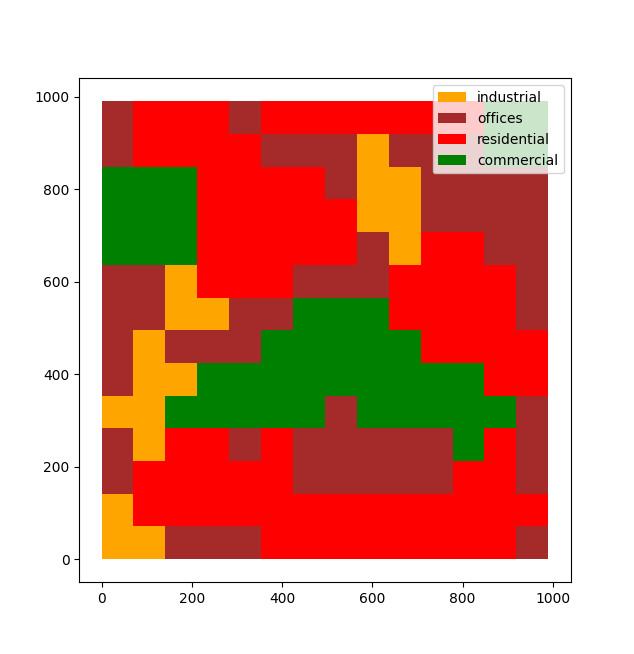
\includegraphics[width=0.45\textwidth]{images/finalzoning.png}
        \caption{Final iteration of zoning}
        \label{fig:final-zoning}
    \end{figure}

    \quad Figure \ref{fig:final-zoning} represents a much more accurate representation of a city layout. The zones are connected via DFS, as seen in Section \ref{zoning}. However, these cells are also a lot smaller. This is because, the size of a cell is now simply the maximum building size. This is still a limitation, but it allows for a much better resolution of the city. The district size is calculated with the same formula as noted above, but not the number of cells in a district are also noted. These are calculated as follows:

    \[C = A \div m\]

    In this formula, C represents the maximum number of cells in a given district, A is once again the district area determined above, and m is the minimum building size of all given zones.

    \subsection{Network Iterations}

    \quad Zones weren't the only aspect of the project to go through many iterations. In fact, the network was modified and redone everytime the zoning structure changed. Each modification came with advancements that allowed it to become a practical and easy to change road system.

    \begin{figure}[H]
        \centering
        \vspace{-1em}
        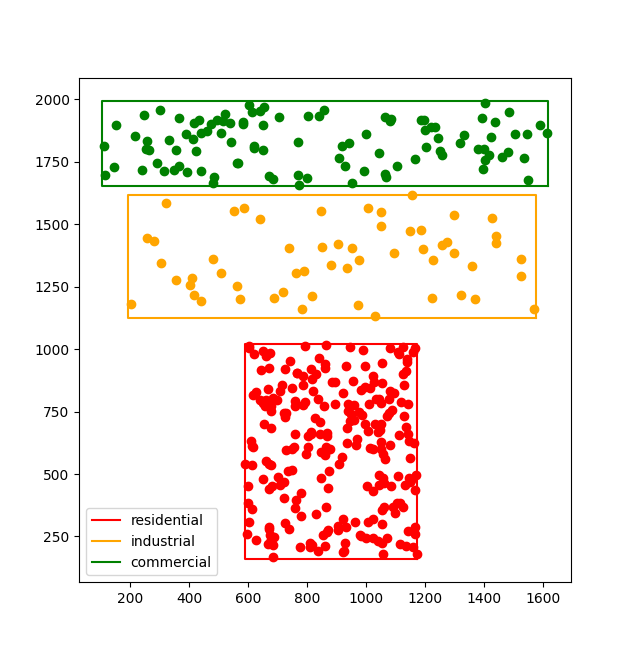
\includegraphics[width=0.45\textwidth]{images/firstzoningwnodes.png}
        \caption{First iteration of network}
        \label{fig:first-network}
    \end{figure}

    \quad As seen in Section \ref{zoning-implementation}, the first zoning implementation did not utilize all available land. Similarly, the nodes created were just randomly generated points within our zone rectangles. Fortunately, there were some configurations that created a modifiable node system. The number of nodes in a zone was defined by the following formula:

    \[N = A \div B\]

    In this formula, N is the number of nodes, A is the area of a district\footnote{The district in this iteration was just a rectangle}, and B is the area of one average building in the zone. Thus, each zone had a different density of dots within it.

    \begin{figure}[H]
        \centering
        \vspace{-1em}
        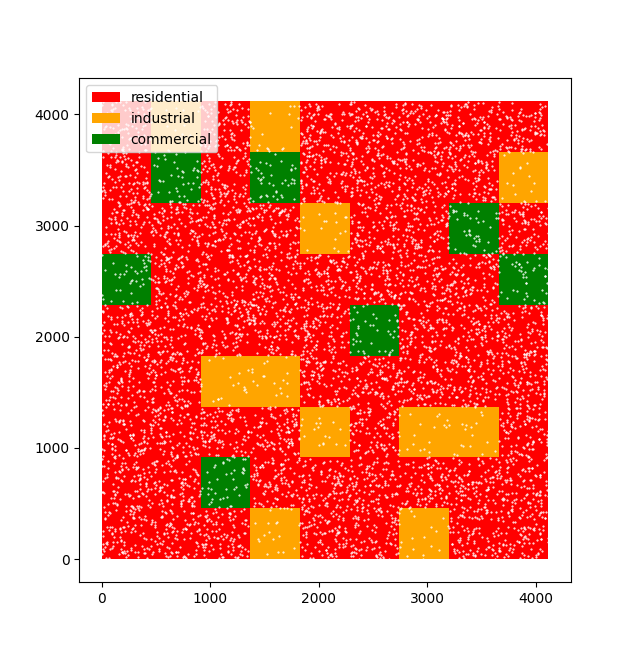
\includegraphics[width=0.45\textwidth]{images/secondzoningwnodes.png}
        \caption{Second iteration of network without roads}
        \label{fig:second-nodes}
    \end{figure}

    \begin{figure}[H]
        \centering
        \vspace{-1em}
        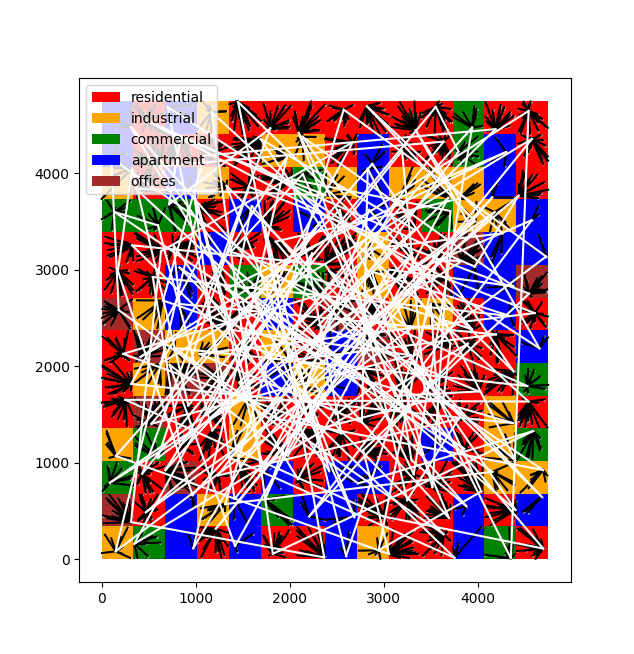
\includegraphics[width=0.45\textwidth]{images/secondzoningwnetwork.png}
        \caption{Second iteration of complete network with roads}
        \label{fig:second-network}
    \end{figure}

    \quad As seen in Figure \ref{fig:second-nodes} the distribution of buildings stayed relatively similar to the previous iteration. The only difference was in the display of them to the user. The larger dots in the previous iteration made the detail of their location less precise. Thus, a reduction of size was a simple fix to make the data more clear. In Figure \ref{fig:second-network} it can be seen that roads are finally implemented. However, this is not very representative of a real city's road system. The reason for this is because of the way roads are assigned. In each district, one central hub is chosen, and every other node is connected to that hub with a district road. These district roads were not configurable and only allowed cars to travel on them. In addition, the mess of white lines is just a very inefficient highway system. In this case, the central hubs are shuffled and connected to the next hub in a list. Despite the ineffective nature of the road network, it still functioned to complete one of the fundamental goals: having a system that allowed a person to move from one building to another. This data was ported onto MATSIM\cite{matsim}, but it did not reveal anything surprising or interesting. \\

    \begin{figure}[H]
        \centering
        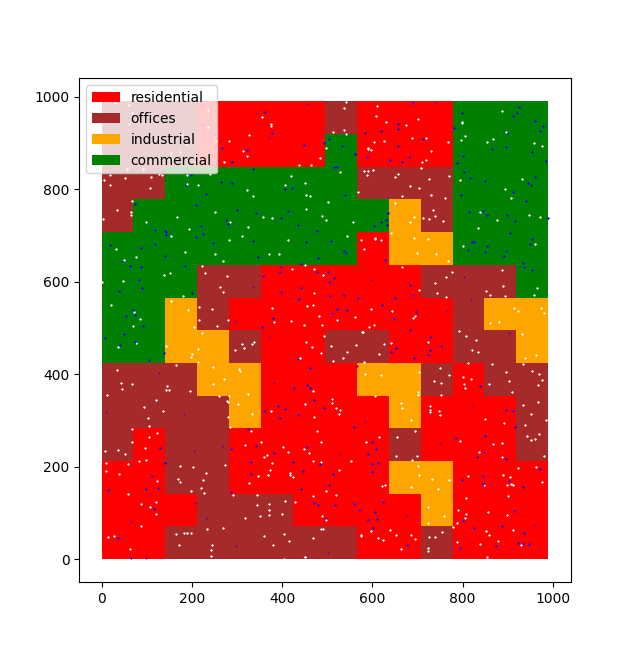
\includegraphics[width=0.45\textwidth]{images/finalzoningwnodes.png}
        \caption{Final iteration of the nodes}
        \label{fig:final-zoning-nodes}
    \end{figure}

    \begin{figure}[H]
        \centering
        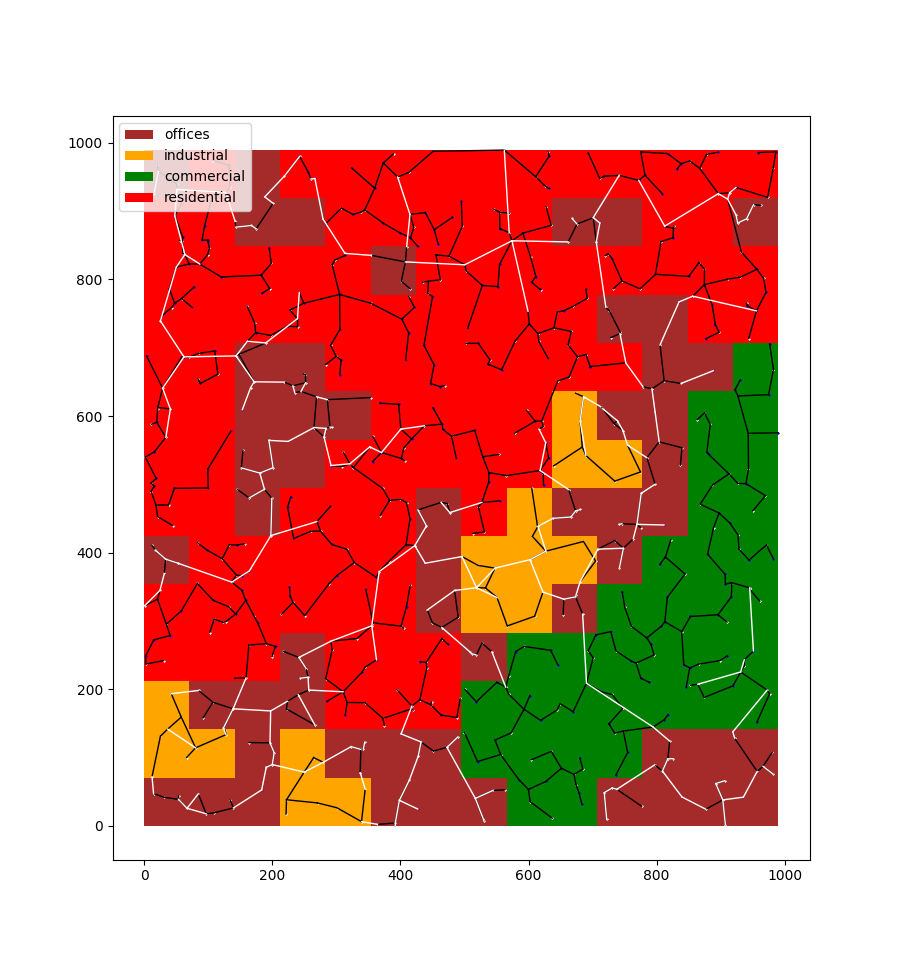
\includegraphics[width=0.45\textwidth]{images/finalnetwork.png}
        \caption{Final iteration of the network}
        \label{fig:final-network}
    \end{figure}

    \quad The final iteration of the road system was much neater and more organized with the help of object oriented programming. The nodes were finally calculated with a different algorithm. Given a district, with a size determined in Section \ref{zoning-implementation}, the land was iterated over to find the placement of zones. The program continuously picked random points in the districts and subtracted the area of the placed building from the remaining area in the district. For a zone with subzones within it, the program simply chose the building type from a list of all possible buildings. Once, again all of this information was configurable by the user. In addition, the program placed atleast one building from the top level zone in this case by checking neighbors within the district for a building of the correct type. If no building was found, then the program inserted a top level building automatically. This resulted in the variation of dot colors as seen in the plot. The different color represent different building types. Finally, this iteration also added our better road network. This was heavily described in section \ref{network}. However, to put it simply the baseline road network is just a minimum spanning tree that connects nodes in a district. The highways are a minimum spanning tree that connect a number of central hubs in each district, defined in the configuration file. Each type of road also has attributes of speed, capacity, and number of lanes, which can be changed by configurations as well. 

    \begin{figure}[H]
        \centering
        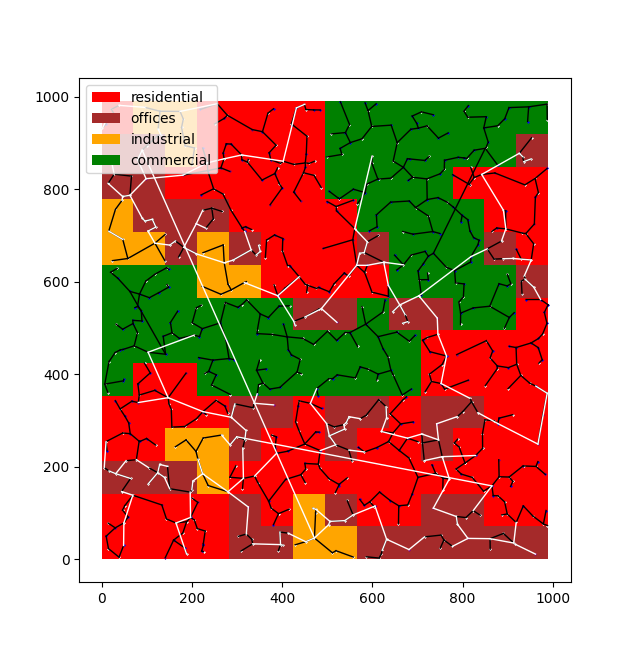
\includegraphics[width=0.45\textwidth]{images/meshednetwork.png}
        \caption{Final iteration of the network with a 1\% meshing ratio}
        \label{fig:final-meshed-network}
    \end{figure}

    \quad The final change made to the network was meshing\footnote{Adding additional roads to the baseline network}. Meshing determined the number of extra roads with the following equation:

    \[R = r \cdot M\]

    In this equation, R represents the number of additional roads, r is the number of existing roads in a district or highway network, and M is the meshing ratio defined by the configuration file. Once the number of additional roads is determined, the algorithm goes through all edges that have not been added to the minimum spanning tree from the complete graph\footnote{A graph with all possible edges} and randomly chooses roads to add to the network till the R value has been satisfied. 

    \subsection{Agent Scheduling}

    \quad The final step of the traffic demand generation is creating the people or agents. These agents require schedules to fulfill the requirements of MATSIM\cite{matsim}. Each schedule must be realistic and also highly configurable. To do this, the program takes in inputs of timings of each activity in particular zones. Thus, when nodes are generated and converted to Location objects, as seen in Section \ref{network}, they also are randomly assigned values of times for when agents use the facilities. In addition, the configuration file also determines the number of workers within each zone. Finally, the configuration file also determines the percentage of people that work from within their district and the percentage of people that work from home. These pieces of data are essentially sifted through with if statements to determine the timings of a person's job. However, to first assign an agent a location to work is a little more complicated. First, for each household, all jobs nearby are sorted from closest to furthest. Then, each location is assigned a weight based on its proximity or index. Finally, the algorithm chooses a random job with the weights assigned. A person is determined to work at home by checking if a random quantity in the range \([0, 1)\) is less than the ratio of the population that work from home. If so, the step of picking a job is skipped. Finally, agents are put through an infinite loop, which has a third of a chance to end every iteration. This loop adds leisure activities after work that fit into the schedule of the agent. These activities are chosen the same way as work. However, this time the number of workers working at the facility does not matter. To increase diversity in schedules, the variability of a person arriving to and leaving from a location can also be modified. Since buildings can have multiple types, people can work and leisure at the same location. This allows for a completely customizable schedule of times and places.

    \begin{figure}[H]
        \centering
        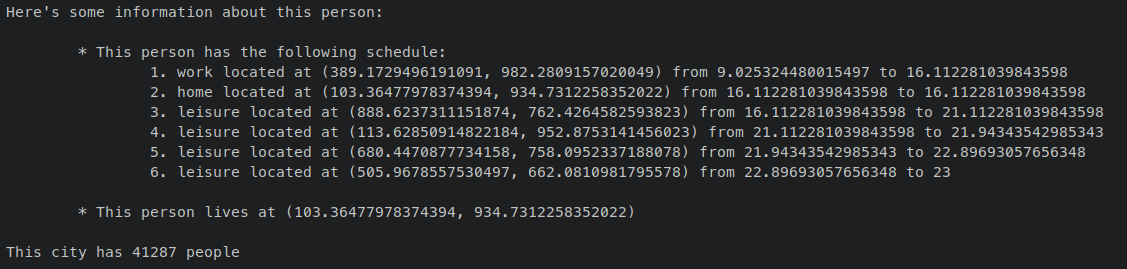
\includegraphics[width=0.4\textwidth]{images/examplepopulation.png}
        \caption{Example schedule of a person}
        \label{fig:example-schedule}
    \end{figure}

    \quad To determine the number of times to create a person, the housing locations\footnote{One building could hold multiple housing locations within it depending on its houseEquivalence value} are iterated through. Each housing location, is assigned a number of residents based on the configuration data. The house is also assigned a number of cars to it also based on the configurations. Finally, the schedules of each person within the household are constructed. If a car isn't available for a person to travel with, they are assigned a bike. In addition, if a car's availability changes throughout the day, a person may come home and take the car to their next location. \\
    
    \section{Simulation}

    \quad Once the traffic demand has been generated, the information can be utilized to simulate the city. As mentioned prior, MATSIM \cite{matsim} is the agent based model of choice for this program. The data produced is converted into XML format for the simulation. These files are stored within the output/ directory and can be used by MATSIM later on. In fact, the code even automatically executes the simulation if the executable file is found in the main directory. These results are stored in the new outputs/ directory and can be analyzed for research. In fact, most of this information can be fed into a wrapper script for implementation of a machine learning algorithm. Such an algorithm can stochastically change the configurations and find the effects on traffic. Simultaneous Perturbation Stochastic Approximation is an example of such an algorithm to find a more ideal city from a starting slate. However, with such a large set of configuration options, a Simulated Annealing algorithm may work better. Despite this, the data from a random city can be found in the figures below.

    \begin{figure}[H]
        \centering
        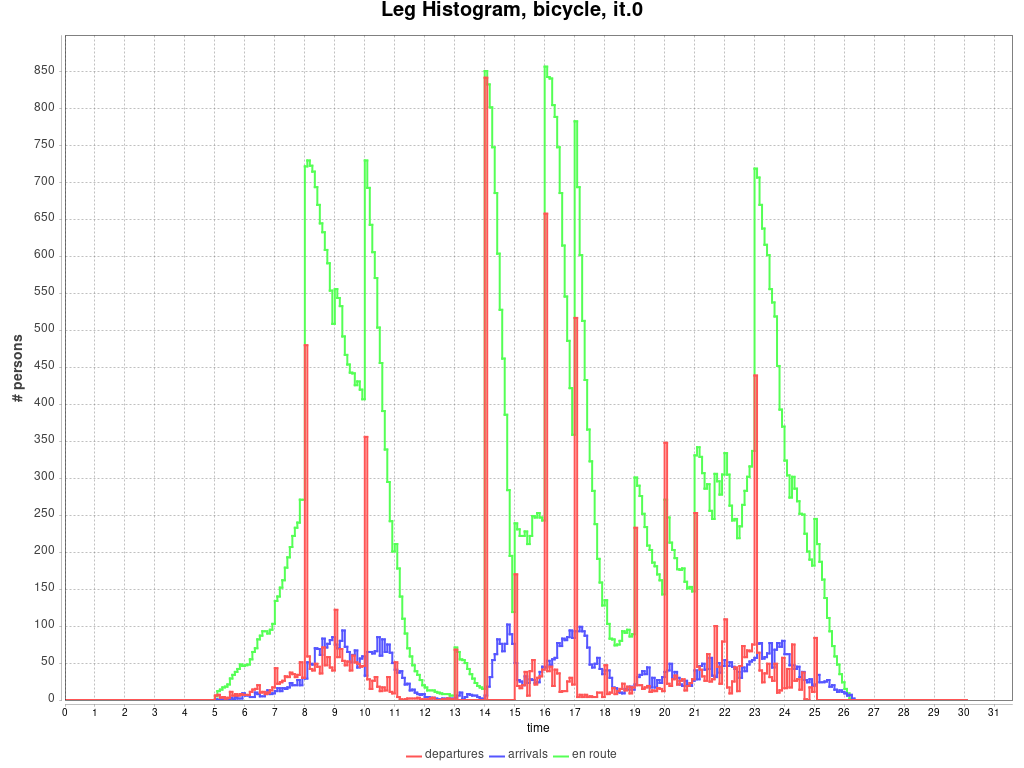
\includegraphics[width=0.45\textwidth]{images/legHistogram.png}
        \caption{Leg histogram example}
        \label{fig:leg-histogram}
    \end{figure}

    \quad The leg histogram found in Figure \ref{fig:leg-histogram} is one of an inefficient city. Nonetheless, it enunciates the different values and makes it clear the meaning of the colors. The red lines represent agents departing from their source locations for any new task in the schedule. The green lines are the number of agents on route. Finally, the blue lines are the number of agents arriving at their destinations. Since this simulation was of a configuration that restricted the bike's speed to 0.5 meter per second, the people took a long time to reach their destinations. It is also clear that due to the few number of jobs in this city, many agents are leaving at around the same time to get to work, however, the schedules in the evenings get a lot more sparse. \\

    \quad Though MATSIM offers several graphs to interpret the data, another important chart shows the distribution in modes of transport. It is clear in the graphs that though biking takes longer, as the hours biked is significantly greater than hours driven, driving is done for about the same distance as biking. The meaning of the different bars is MATSIM's own stochastic changes to a population. This allows the user to see how much a population would change from the norm and if the findings are a coincidence or have a strong correlation.

    \begin{figure}[H]
        \centering
        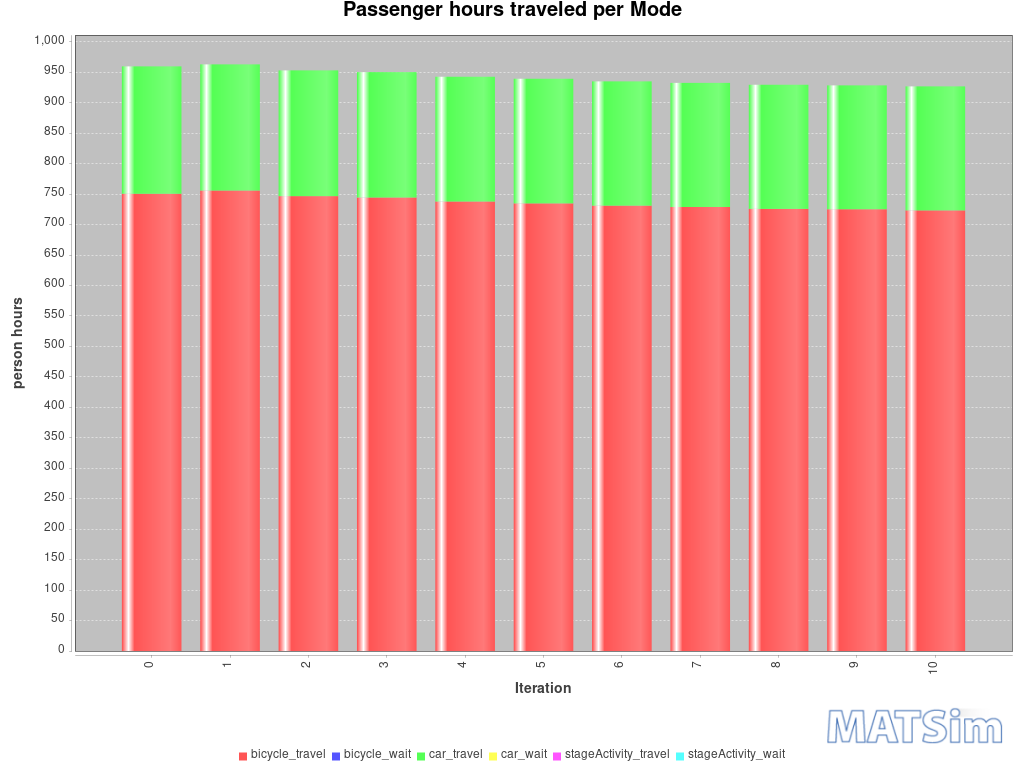
\includegraphics[width=0.45\textwidth]{images/phModestats.png}
        \caption{Hours mode stats example}
        \label{fig:ph-modestats}
    \end{figure}

    \begin{figure}[H]
        \centering
        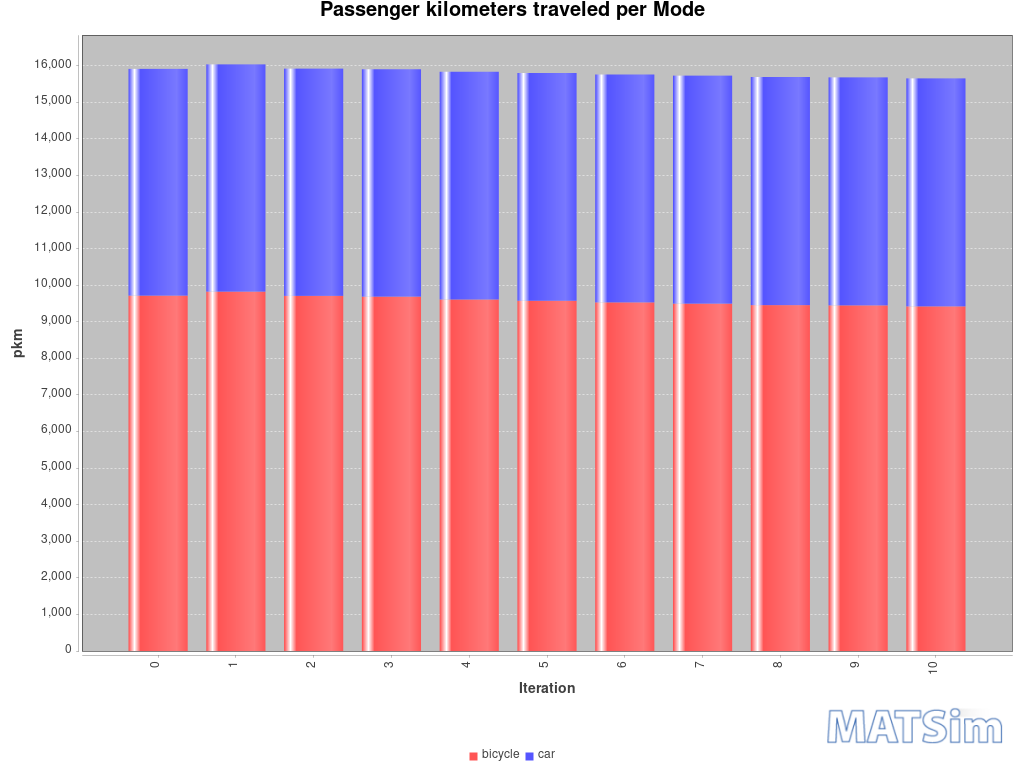
\includegraphics[width=0.45\textwidth]{images/pkmModestats.png}
        \caption{Distance modestats example}
        \label{fig:pkm-modestats}
    \end{figure}

    \section{Conclusion}

    \quad This project was successful in that it captured and modeled a theoretical city from a very easily configurable json file. Of course, there are always things that can be done better. For one, the zoning policy is enforced on pixels that are the size of the largest possible buildings. However, this doesn't work in all cases. Sometimes, housing zones may take up less space than one industrial building. To account for this, a better system of DFS needs to be implemented to ensure that each zone can break down to different size cells. In addition, one of the major flaws of this program is multi-modal transportation. Though, the pipeline does take biking and cars into account, a network of public transport systems would be an amazing update for traffic engineers. The only difficulty with this is allowing the user to easily configure the timings of each public transport line. Despite these setbacks, the project went through several iterations and does a great job of capturing some of the most complex details of a city. Along with fitting in smoothly with MATSIM, the project can be very much added upon with a wrapper stochastic approximation script. This could reveal aspects of city design that may not be known about yet.

    \section*{Acknowledgement}
    We would like to thank \textbf{The Institute for Computing in Research} for this wonderful opportunity to research such a fascinating topic.
\end{multicols}

\pagebreak

\bibliography{bibliography}
\bibliographystyle{ieeetr}

\end{document}
